\documentclass[conference,letterpaper,10pt]{IEEEtran}

\usepackage{cite}
\usepackage{amsmath,amssymb}
\usepackage{graphicx}
\usepackage{booktabs,multirow,array}
\usepackage{microtype}
\usepackage[hidelinks]{hyperref}
\urlstyle{same}
\hyphenation{Deep-Seek multi-turn}
\emergencystretch=1em
\setlength{\textfloatsep}{4.0pt plus 1.0pt minus 1.0pt}
\setlength{\dbltextfloatsep}{4.0pt plus 1.0pt minus 1.0pt}
\setlength{\dblfloatsep}{3.5pt plus 1.0pt minus 1.0pt}
\setlength{\abovecaptionskip}{2.0pt plus 0.8pt minus 0.8pt}
\renewcommand{\dbltopfraction}{0.92}
\renewcommand{\topfraction}{0.92}
\renewcommand{\textfraction}{0.06}
\renewcommand{\floatpagefraction}{0.88}
\renewcommand{\dblfloatpagefraction}{0.88}
\setcounter{dbltopnumber}{2}
\setcounter{topnumber}{2}
\setcounter{totalnumber}{3}

% ---- unified protocol / regime names (used everywhere: text, tables, figures) ----
\newcommand{\pFULL}{\texttt{FULL}}
\newcommand{\pCON}{\texttt{CONCAT}}
\newcommand{\pCONM}{\texttt{CONCAT-M}}
\newcommand{\pFREE}{\texttt{FREE}}
\newcommand{\pREQ}{\texttt{REQ}}
\newcommand{\pGRD}{\texttt{GUARD}}
\newcommand{\TA}{TypeA}
\newcommand{\TB}{TypeB}

\begin{document}

\title{Certified Insufficiency and Premature Commitment:\\Process--Outcome Evaluation of Reasoning LLMs\\under Progressive Information Disclosure}

\IEEEoverridecommandlockouts
\author{%
\IEEEauthorblockN{Weike Cai\textsuperscript{1,*}, Mohan Tang\textsuperscript{2,*}}
\IEEEauthorblockA{\textit{\textsuperscript{1}School of Mathematics, Sichuan University, Chengdu, China}\\
\textit{\textsuperscript{2}School of Mathematics and Statistics, Central China Normal University, Wuhan, China}\\
caiweike@stu.scu.edu.cn, tangmohan@mails.ccnu.edu.cn}
\thanks{\textsuperscript{*}Both authors contributed equally to this work and share first authorship.}
}

\maketitle

\begin{abstract}
In computer-supported collaborative design, requirements reach an AI assistant incrementally, yet benchmarks usually score only final-turn accuracy ($Y$), crediting unsupported answers before premises suffice---\emph{premature commitment} ($E$). We study this failure on a frozen 120-problem OlympiadBench benchmark whose SymPy leave-one-out certificates check clause necessity on formalized constraints, separating a strictly underdetermined core (\TA) from a relaxed-extremum set (\TB) admitting locally valid but unscoped answers. Evaluating 5,400 trajectories from three open-weight reasoning models across six paired protocols with two input-blind LLM judges, SymPy grading, and a 3-rater blind audit (one external, no adjudication), we find: (1)~on \TA{} under \pFREE{} and \pREQ, $10.3\%$--$18.6\%$ of trajectories commit prematurely, so $9.3\%$--$17.2\%$ end correct despite an earlier premature commit ($Y{-}J$); (2)~first-commit hazard rises sharply in later turns (odds ${\times}2.3$/turn within fixed task depth); (3)~unprompted retraction is rare: judges flag $0.8\%$--$5.3\%$ of 489 committed trajectories, and human raters confirm $[0,1]/26$ flagged candidates and $0/74$ sampled controls ($0/50$ audited \TA); and (4)~an exploratory Turn-1 uniqueness guard reduces unconditional \TA{} commits only suggestively when pooled ($-2.6$ to $-2.9$~pp) and not on \TB{}, partly shifting replies to conditional scope (null on \texttt{Commit}+\texttt{Conditional} and holding mainly on \texttt{Qwen3-14B}). These controlled findings motivate testing completeness cues and explicit retractions with human collaborators.
\end{abstract}

\begin{IEEEkeywords}
human--AI collaboration; collaborative design; progressive information disclosure; premature commitment; information sufficiency; reasoning LLMs.
\end{IEEEkeywords}

\section{Introduction}

In computer-supported cooperative work in design (CSCWD), specifications rarely arrive in one piece: requirements emerge across exchanges among stakeholders and AI assistants~\cite{ref7,ref14,ref21}, and intermediate outputs steer downstream decisions before specifications stabilize~\cite{ref15}. Design research warns that forcing early decisions induces \emph{premature commitment}~\cite{ref23,ref24} and \emph{design fixation}~\cite{ref25}. Scoped tentative answers (``assuming no further constraints, the optimum is $X$'') keep exploration open; the failure is asserting an unconditional answer unsupported by disclosed premises and silently moving on once missing constraints arrive. Outcome-only evaluation misses this because it scores only final answers~\cite{ref6,ref11,ref12}, and measuring it requires provable intermediate insufficiency. We therefore use competition math under scripted passive disclosure as a \emph{certifiable controlled baseline} for incremental specification: clauses stand in for stakeholder requirements, and symbolic certificates check clause necessity on formalized constraints so no intermediate turn fixes the answer, motivating interactive safeguard tests with real collaborators.

Consider sequence task \texttt{ob-comp-416} (\TA, six turns). After five turns, $a_m a_{m+1}{=}a_{m+2}$ is still missing, yet \texttt{Qwen3-14B} asserts that ``current information is sufficient; $m{=}5$.'' Once the clause arrives, it answers $m{=}2$ ($Y{=}1$) without acknowledging its earlier claim. Outcome scoring records a success, whereas a collaborator acting on Turn~5 locked in a wrong value never flagged for reversal. We separate $Y$, $E$, joint success $J{=}Y(1{-}E)$, and unprompted retraction---measuring assistant-side recovery preconditions while leaving to user studies whether explicit retraction aids collaborator revision after early adoption.

Prior multi-turn studies~\cite{ref1,ref4} face two obstacles: (i)~unverified prefixes risk penalizing deduction from redundant clauses or conflating unidentifiable states with locally well-posed relaxed optima; and (ii)~comparing canonical prompts to permuted histories confounds rewriting, ordering, and interaction. We solve (i) via symbolic necessity certificates separating \TA{} (every prefix underdetermined) from \TB{} (prefixes may admit a valid relaxed optimum needing scope qualification) and (ii) via paired controls:
\begin{itemize}
    \item \textbf{RQ1:} How large is $Y{-}J$ under progressive disclosure after controlling for rewriting/ordering, and does it persist on \TA?
    \item \textbf{RQ2:} When do first commits occur, and how do current-answer requests shift scope (\texttt{Wait} vs.\ \texttt{Conditional})?
    \item \textbf{RQ3:} When decisive clauses arrive, how often do models retract earlier commits unprompted?
    \item \textbf{RQ4:} Does a Turn-1 uniqueness guard lower $E$, and does its effect differ across \TA{} and \TB?
\end{itemize}

Contributions: (1)~a 120-problem benchmark with SymPy-checked certificates separating \TA/\TB{} (Sec.~\ref{sec:benchmark}); (2)~a six-protocol paired study across three reasoning models (5,400 trajectories; Sec.~\ref{sec:method}--\ref{sec:exp2}); (3)~a hazard and retraction audit (Sec.~\ref{sec:exp3}); and (4)~an exploratory Guard$\times$regime test with a 3-rater 100/100 \textsc{Test} certificate census and blind scope/retraction audits (Sec.~\ref{sec:exp4b}--\ref{sec:exp4a}). Artifacts: \url{https://github.com/caiweike/certified-insufficiency}.

\section{Related Work}

\textbf{Multi-turn underspecification and clarification.} Laban et al.~\cite{ref1} showed accuracy drops when tasks unfold across turns, motivating view-asymmetric distillation~\cite{ref2} and abstention-reward curriculum RL~\cite{ref3}. Clarification benchmarks test disambiguation and post-clarification answering~\cite{ref4,ref5}; QuestBench~\cite{ref27} tests identifying a single missing variable, and missing premises exacerbate overthinking~\cite{ref28}. Most closely, MT-InfoSeek~\cite{ref29} studies multi-turn sufficiency, answer timing, and final-accuracy decoupling during active querying on $k$-underspecified tasks. Selective QA~\cite{ref8,ref9,ref10} studies single-turn abstention, and LLMs rarely self-correct unprompted~\cite{ref26}. Beyond MT-InfoSeek, four designs add measurable structure: (i)~SymPy certificates ensuring insufficiency across \emph{every} prefix/order (filtering 86 redundant items for paired order controls); (ii)~\TA/\TB{} semantics separating strict underdetermination from relaxed optima; (iii)~passive \texttt{Commit}/\texttt{Conditional}/\texttt{Wait} scoping; and (iv)~retraction auditing.

\textbf{Commitment in design and human--AI collaboration.} Cognitive Dimensions defines premature commitment as forcing decisions before information is ready~\cite{ref23,ref24}; design fixation captures early anchoring~\cite{ref25}. We study the AI-side analogue in multi-round LLM design~\cite{ref21}, extending mixed-initiative guidelines for conveying uncertainty and supporting correction~\cite{ref7,ref14,ref15}. Reasoning LLMs (Qwen3~\cite{ref16}, GLM~\cite{ref17}) excel via long CoT~\cite{ref13,ref6}, yet outcome accuracy misses these process risks.

\section{Formally Certified Benchmark}\label{sec:benchmark}

We start from the 1,648 Chinese competition and CEE text-only open-ended problems in \textsc{OlympiadBench}~\cite{ref6} (408 competition, 1,240 CEE).

\subsection{Eligibility Filtering and Stratification}
An offline filter (rules \texttt{v2.4.0}) removes structurally invalid ($-499$), non-constraining, extraneous, or audit ($-30$), out-of-range clause-count ($k{\notin}[3,6]$, $-229$), and near-duplicate ($-249$) items, leaving 641 singletons. Stratified sampling (seeds 2026/2027) assigns 100 provisional \textsc{Test}, 20 \textsc{Dev}, and 521 reserve items across four topic groups---Functions/Calculus/Trig (G1), Algebra/Inequalities (G2), Sequences/Combinatorics/NT (G3), Geometry/Analytic (G4)---and two regimes.

\subsection{Symbolic Certificates and Two Regimes}
Each item is split at exact character spans into an opening stem/target $S_1$ and condition clauses $\{S_2,\dots,S_k\}$, $k\in\{3,\dots,6\}$. An LLM proposes a formalization and certificates, which SymPy~\cite{ref19} checks: the full clause set must be satisfiable and reproduce the official answer, and every $S_j$ ($j\ge2$) must be \emph{necessary}:
\begin{itemize}
    \item \textbf{\TA{} (unique value; strict underdetermination).} A \texttt{WitnessPair}: two assignments satisfying all clauses except $S_j$ with distinct target values. Any prefix missing $S_j$ imposes a subset of those constraints, so the witness pair remains feasible for \emph{every} prefix and \emph{every} disclosure order: no non-final turn determines the answer. For example, in \texttt{ob-cee-3984} (target $\tan(\alpha{-}\frac{\pi}{4})$, $S_2$: $\cos\alpha{=}\frac{1}{3}$, $S_3$: Quadrant~IV), the full witness $\alpha{=}{-}\arccos\frac{1}{3}$ yields $\frac{9+4\sqrt2}{7}$, while dropping $S_2$ admits $\alpha{=}{-}\frac{\pi}{6}$ ($-2{-}\sqrt3$) and dropping $S_3$ admits $\alpha{=}\arccos\frac{1}{3}$ ($\frac{9-4\sqrt2}{7}$).
    \item \textbf{\TB{} (extremum or range; relaxed scoping).} Each $S_j$ needs a relaxed certificate (\texttt{RelaxedCertificate}): an assignment satisfying all clauses except $S_j$ whose objective strictly beats or escapes the full-task extremum or range. Some relaxed prefixes still have a finite, unique optimum (e.g., $\max(\sin A{+}\sin B{+}\sin C){=}\tfrac{3\sqrt3}{2}$), so a \TB{} ``commit'' may correctly solve the relaxed task while omitting scope qualification; we thus treat \TB{} $E$ as an \emph{unscoped-answer} rate and base primary claims on \TA.
\end{itemize}

Stage~2 audited 364 candidates and rejected 244 (67.0\%: 90 alignment, 86 redundant-premise, 45 missing-certificate, 15 answer-key, 8 regime), freezing \texttt{verified\_120\_v1}: 81 \TA{} (68 \textsc{Test}, 13 \textsc{Dev}) and 32 \TB{} \textsc{Test} items (G1 19/10, G2 13/10, G3 21/3, G4 15/9; $k{=}3/4/5/6$: 44/34/16/6, mean $3.84$). As SymPy checks formalized constraints rather than Chinese prose, three blind raters (two authors, one external; \texttt{SEED=2026}, no adjudication) scored all 100 \textsc{Test} items (852 prefixes) as Faithful/Minor/Unfaithful. Across $[L,U]$ bounds (prioritized over majority as two raters are authors), strict fidelity varies across Minor thresholds ($[75,100]/100$: per-rater $79/94/99$, majority $97$; $83.3\%$ agree, $\mathrm{AC1}{=}0.80$, $\kappa{=}{+}0.02$), whereas necessity holds more consistently on $[91,100]/100$ ($92/100/99$, majority $100$: \TA{} $[63,68]$, \TB{} $[28,32]$; $94.0\%$ agree, $\mathrm{AC1}{=}0.94$, $\kappa{=}{-}0.03$~\cite{ref20}; external--author $95.0\%$ vs.\ $92.0\%$). Two \TA{} items (\texttt{ob-cee-4352}, \texttt{ob-cee-3282}) receive single-rater prefix-flip flags ($[0,2]/100$ items, $[0,4]/852$ prefixes, majority $0$, $\mathrm{AC1}{=}0.99$, $\kappa{=}{-}0.01$; $0/32$ \TB): dropping those two shifts dynamic $E_L,E_U,Y{-}J_L$ by ${\le}0.26$~pp (${\le}0.43$~pp on \TA), and dropping all 9 items marked Unfaithful by any rater shifts dynamic $E_L,E_U$ by ${-}1.35/{-}1.42$~pp (${-}1.22/{-}1.37$~pp on \TA{} \pFREE/\pREQ, leaving \TA{} $E$ at $9.0\%$--$16.9\%$). \TA--\TB{} contrasts remain associational because topic, depth, and baseline $E$ differ.

\section{Paired Protocols, Metrics, and Judging}\label{sec:method}

\subsection{Models and Decoding}
We evaluate Qwen3-8B, Qwen3-14B~\cite{ref16}, and GLM-Z1-9B-0414~\cite{ref17} at pinned HuggingFace revisions in BF16 via vLLM~\cite{ref18} using native thinking templates (temperature 0.6, top-$p$ 0.95, 16,384 output / 32,768 context tokens). Turn-1 rules are shared; history keeps visible replies only (max context 19,286 tokens). On \textsc{Dev}~20, 16K cut empty truncations to 1--2\% vs.\ 4K--8K.

\subsection{Six Strictly Paired Protocols}
Each \textsc{Test} item runs $R{=}3$ reps/protocol (300 trajectories, 852 turns/cell; 5,400 total): Rep~0 canonical, Reps~1--2 shared permutations of $\{S_2,\dots,S_k\}$ ($S_1$ fixed). Protocols: (1)~\pFULL{} (original single-turn); (2)~\pCON{} (clauses concatenated canonically); (3)~\pCONM{} (each rep's order); (4)~\pFREE{} (one clause/turn; Turn-1 notes more conditions may follow); (5)~\pREQ{} (\pFREE{} + per-turn current-answer/basis prompt); (6)~\pGRD{} (\pREQ{} + Turn-1 instruction to verify uniqueness before unconditional/\verb|\boxed{}| answers, else wait or state assumptions). The final turn states all clauses are given.

\begin{figure}[!t]
    \centering
    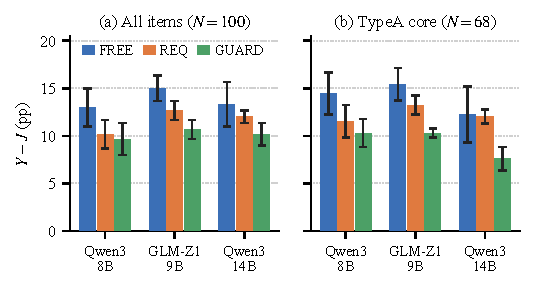
\includegraphics[width=\columnwidth]{fig1_yj_gap.pdf}
    \caption{Process--outcome gap $Y{-}J$ (= share of trajectories that are finally correct but committed prematurely) in the three multi-turn protocols. Bars: midpoint; whiskers: dual-judge $[L,U]$ bounds. Single-turn controls have $Y{-}J\equiv0$. Final accuracy remains high ($85.0\%$--$92.7\%$ overall, $90.7\%$--$99.0\%$ on \TA; Tables~\ref{tab:main_results}, \ref{tab:exp3_mechanism}).}
    \label{fig:y_vs_j}
\end{figure}

\subsection{Metrics and Inference}
For item $i$, protocol $c$, rep $r$, and turn $t<k_i$, certificates fix ground truth ``insufficient''. A judge labels each non-final reply as \texttt{Wait}, \texttt{Conditional} (bound to stated assumptions), \texttt{Commit} (unconditional), \texttt{Partial/Other}, or \texttt{Unresolved}. Turn commit bounds $[\underline e,\overline e]$ are $[1,1]$ (\texttt{Commit}), $[0,1]$ (\texttt{Unresolved} or judge split), and $[0,0]$ otherwise. Trajectory bounds are
\begin{equation}
\underline{E}_{icr} = \max_{t < k_i} \underline{e}_{icrt}, \qquad
\overline{E}_{icr} = \max_{t < k_i} \overline{e}_{icrt},
\end{equation}
so $E_L$ counts commits confirmed by both judges and $E_U$ commits flagged by either. With final-accuracy bounds $[\underline Y,\overline Y]$, $J{=}Y(1{-}E)$ has bounds $[\underline Y(1{-}\overline E),\,\overline Y(1{-}\underline E)]$, and $Y{-}J{=}Y{\cdot}E$ counts premature commits that later end correct. The first-commit hazard is
\begin{equation}
h(t,k) = \mathbb{P}\!\left(e_{icrt}{=}1 \,\middle|\, k_i{=}k,\ \textstyle\max_{s<t} e_{icrs}{=}0\right),
\end{equation}
with remaining clauses $r{=}k{-}t\in\{1,\dots,5\}$. Because $t$ and $r$ are collinear within fixed $k$, we fit $\operatorname{logit} h = \alpha + \beta_t t + \beta_k k + \gamma_{\text{prot}} + \delta_{\text{model}} = \alpha + (\beta_t{+}\beta_k)t + \beta_k r + \gamma_{\text{prot}} + \delta_{\text{model}}$: $\beta_t$ captures the joint per-turn change within fixed $k$ ($+1$ turn, $-1$ remaining clause), $\beta_t{+}\beta_k$ the per-turn slope at fixed $r$, and $\beta_k$ the remaining-clause slope at fixed $t$. Contrasts use 10,000-sample paired item bootstraps (regime-stratified for interactions; item-clustered for hazards), reporting conservative envelopes $[A_L{-}B_U,\,A_U{-}B_L]$ and per-judge 95\% CIs. Without multiplicity correction, protocol contrasts are \emph{significant} only if cross-judge envelope 95\% CIs exclude 0; within-regime Guard contrasts ($\Delta E_{\mathrm{TypeA}},\Delta E_{\mathrm{TypeB}}$) and interactions ($\Delta E_{\mathrm{TypeA}}{-}\Delta E_{\mathrm{TypeB}}$) are \emph{regime-significant} if both $E_L$ and $E_U$ 95\% CIs exclude 0; and effects are \emph{suggestive} if only one bound or per-judge CI does.

\subsection{Dual-LLM Judging}
All 5,400 trajectories are graded by \texttt{gpt-6.1-sol} (primary) and \texttt{deepseek-v4.1-flash} (secondary) at temperature 0, low reasoning effort (Nov.\ 21--22, 2026; caches in repo) for (i)~final correctness/abstention, (ii)~non-final scope, and (iii)~explicit repair on $E_U{=}1$ trajectories (retraction, qualification, or neither). Scope/repair judges are input-blind---seeing only disclosed clauses and visible replies up to turn $t$, never future turns, item IDs, regimes, or protocol rules (Guard echoes $<0.5\%$). Rubrics froze on \textsc{Dev}~20 ($\kappa_Y{\ge}0.90$, pooled $\kappa_E{\ge}0.85$, 0 parse failures).

\begin{table*}[!t]
\centering
\caption{Main results on \textsc{Test}~100 (100 problems $\times$ 3 reps = 300 trajectories per cell). $[L,U]$: dual-judge bounds (single value when $L{=}U$). $Y$: final accuracy; $E$: premature commitment on insufficient turns; $J{=}Y(1{-}E)$; $Y{-}J$: finally correct trajectories that committed prematurely.}
\label{tab:main_results}
\footnotesize
\setlength{\tabcolsep}{4.0pt}
\renewcommand{\arraystretch}{0.94}
\begin{tabular}{@{}llcccccccc@{}}
\toprule
Model & Protocol & $Y$ (\%) & $E$ (\%) & $J$ (\%) & $Y-J$ (\%) & $P(E{=}1\mid Y{=}1)$ & Abstain (\%) & Trunc. (\%) & Tok./Traj \\
\midrule
\multirow{6}{*}{Qwen3-8B} & \pFULL & 94.0 & 0.0$^*$ & 94.0 & 0.0 & 0.0 & 0.3 & 3.3 & 4,959 \\
 & \pCON & 94.7 & 0.0$^*$ & 94.7 & 0.0 & 0.0 & [0.3, 0.7] & 3.0 & 4,956 \\
 & \pCONM & 93.7 & 0.0$^*$ & 93.7 & 0.0 & 0.0 & 0.3 & 3.0 & 4,931 \\
 & \pFREE & 87.7 & [17.0, 21.7] & [72.7, 76.7] & [11.0, 15.0] & [12.6, 17.1] & 0.7 & 1.7 & 12,875 \\
 & \pREQ & [85.3, 86.3] & [13.7, 17.0] & [74.0, 77.7] & [8.7, 11.7] & [10.0, 13.6] & 2.0 & 2.0 & 10,713 \\
 & \pGRD & [86.7, 87.0] & [13.3, 16.7] & [75.3, 79.0] & [8.0, 11.3] & [9.2, 13.1] & [2.0, 2.3] & 1.3 & 10,301 \\
\midrule
\multirow{6}{*}{GLM-Z1-9B} & \pFULL & [94.3, 94.7] & 0.0$^*$ & [94.3, 94.7] & 0.0 & 0.0 & 1.0 & 1.7 & 3,617 \\
 & \pCON & 93.7 & 0.0$^*$ & 93.7 & 0.0 & 0.0 & 1.7 & 0.7 & 3,346 \\
 & \pCONM & 92.0 & 0.0$^*$ & 92.0 & 0.0 & 0.0 & 1.7 & 0.7 & 3,290 \\
 & \pFREE & [87.3, 88.0] & [17.7, 21.3] & [71.3, 74.0] & [13.7, 16.3] & [15.6, 18.6] & [3.3, 3.7] & 0.3 & 10,514 \\
 & \pREQ & [85.3, 86.0] & [15.0, 18.0] & [72.0, 74.0] & [11.7, 13.7] & [13.6, 16.0] & 5.0 & 1.7 & 9,076 \\
 & \pGRD & [85.0, 85.7] & [14.3, 16.7] & [73.7, 75.7] & [9.7, 11.7] & [11.3, 13.7] & [4.3, 4.7] & 2.7 & 9,401 \\
\midrule
\multirow{6}{*}{Qwen3-14B} & \pFULL & 97.0 & 0.0$^*$ & 97.0 & 0.0 & 0.0 & 0.0 & 2.0 & 5,271 \\
 & \pCON & 96.0 & 0.0$^*$ & 96.0 & 0.0 & 0.0 & 0.3 & 2.0 & 5,022 \\
 & \pCONM & 95.0 & 0.0$^*$ & 95.0 & 0.0 & 0.0 & 0.3 & 2.7 & 5,134 \\
 & \pFREE & [91.7, 92.0] & [14.3, 19.3] & [76.3, 81.0] & [11.0, 15.7] & [12.0, 17.0] & 1.7 & 2.0 & 13,450 \\
 & \pREQ & [92.3, 92.7] & [14.7, 17.0] & [79.7, 81.3] & [11.3, 12.7] & [12.2, 13.7] & 0.0 & 1.3 & 11,180 \\
 & \pGRD & 92.7 & [12.7, 15.3] & [81.3, 83.7] & [9.0, 11.3] & [9.7, 12.2] & [1.7, 2.0] & 0.7 & 10,662 \\
\bottomrule
\multicolumn{10}{@{}l}{\scriptsize $^*$Single-turn controls have no insufficient intermediate turns ($E\equiv 0$ structurally, hence $J\equiv Y$).}
\end{tabular}
\end{table*}


\section{Experimental Results}

\subsection{Controls and the Process--Outcome Gap (RQ1)}\label{sec:exp2}
\textbf{No detectable rewriting or reordering effect.} \pFULL$-$\pCON{} ranges from $-0.7$ to $+1.0$~pp and \pCON$-$\pCONM{} from $+1.0$ to $+1.7$~pp across all three reps (95\% CIs within $[-3.0,+4.3]$~pp; Table~\ref{tab:paired_contrasts}). Because Rep~0 uses canonical order in both \pCON{} and \pCONM{}, restricting \pCON$-$\pCONM{} to permuted Reps~1--2 ($n{=}200$/model) gives $+1.0$ to $+3.0$~pp with 95\% CIs within $[-2.5,+6.0]$~pp (all including zero); smaller order effects remain possible.

\textbf{Disclosure lowers $Y$ modestly but opens a large $Y{-}J$ gap.} Moving from \pCONM{} to \pFREE{} lowers $Y$ by $3.0$--$6.0$~pp (significant for \texttt{Qwen3-8B} only) while raising tokens/trajectory $2.6$--$3.2{\times}$ ($2.0$--$2.4{\times}$ completion; Table~\ref{tab:main_results}). Premature commitment hits $13.7\%$--$21.7\%$ of \pFREE/\pREQ{} trajectories, leaving $8.7$--$16.3$~pp finally correct yet committed early (Fig.~\ref{fig:y_vs_j}a). On the \TA{} core, $E$ is $10.3\%$--$18.6\%$ and $Y{-}J$ is $9.3$--$17.2$~pp despite $90.7\%$--$99.0\%$ final accuracy (Fig.~\ref{fig:y_vs_j}b, Table~\ref{tab:exp3_mechanism}). Among confirmed \TA{} commits boxing answers at both commit and final turns, 36.2\% (46/127) match lexically; excluding all 88 lexically matched trajectories still leaves \TA{} $E_L$ at $8.5\%$--$12.2\%$ and $Y{-}J$ at $7.0$--$14.7$~pp under \pFREE/\pREQ{}, showing the gap is not driven solely by verbatim final-answer recall (non-verbatim recall remains possible; Sec.~VI).

\begin{table*}[!t]
\centering
\caption{Paired problem-bootstrap contrasts on \textsc{Test}~100 (pp, $B{=}10{,}000$). Outcome rows: point range $[L,U]$ and 95\% envelope CI (lo, hi); $^*$CI excludes 0. Interaction rows: $\Delta E_{\mathrm{TypeA}}{-}\Delta E_{\mathrm{TypeB}}$ for \pGRD$-$\pREQ{} (stratified bootstrap), by $E_L$/$E_U$; $^*$CI excludes 0. Scope rows: 95\% envelope CI / primary / secondary; $^\dagger$judge CI excludes 0 (no envelope does). \TA/\TB{} rows give envelopes; per-bound $E_L$/$E_U$ CIs appear in Fig.~\ref{fig:scope_hazard}b and Sec.~\ref{sec:exp4b}.}
\label{tab:paired_contrasts}
\footnotesize
\setlength{\tabcolsep}{4.0pt}
\renewcommand{\arraystretch}{0.96}
\begin{tabular}{@{}lccc@{}}
\toprule
Paired contrast (pp) & Qwen3-8B & GLM-Z1-9B & Qwen3-14B \\
\midrule
\pFULL{} $-$ \pCON{} ($\Delta Y$) & $-$0.7 ($-$3.0, $+$1.3) & [$+$0.7, $+$1.0] ($-$2.3, $+$4.0) & $+$1.0 ($-$1.0, $+$3.7) \\
\pCON{} $-$ \pCONM{} ($\Delta Y$) & $+$1.0 ($-$0.7, $+$3.0) & $+$1.7 ($-$0.7, $+$4.3) & $+$1.0 ($-$0.7, $+$2.7) \\
\pCONM{} $-$ \pFREE{} ($\Delta Y$) & $+$6.0 ($+$2.3, $+$10.0)$^*$ & [$+$4.0, $+$4.7] ($-$0.7, $+$9.7) & [$+$3.0, $+$3.3] ($-$0.3, $+$7.3) \\
\pREQ{} $-$ \pFREE{} ($\Delta Y$) & [$-$2.3, $-$1.3] ($-$6.0, $+$2.0) & [$-$2.7, $-$1.3] ($-$7.0, $+$3.3) & [$+$0.3, $+$1.0] ($-$2.7, $+$4.3) \\
\pREQ{} $-$ \pFREE{} ($\Delta E$) & [$-$8.0, $+$0.0] ($-$12.3, $+$3.7) & [$-$6.3, $+$0.3] ($-$10.0, $+$4.7) & [$-$4.7, $+$2.7] ($-$8.0, $+$5.7) \\
\midrule
\pGRD{} $-$ \pREQ{} ($\Delta E$) & [$-$3.7, $+$3.0] ($-$7.3, $+$6.7) & [$-$3.7, $+$1.7] ($-$8.3, $+$6.0) & [$-$4.3, $+$0.7] ($-$7.7, $+$4.0) \\
\pGRD{} $-$ \pREQ{} ($\Delta J$) & [$-$2.3, $+$5.0] ($-$7.3, $+$10.0) & [$-$0.3, $+$3.7] ($-$5.3, $+$9.0) & [$+$0.0, $+$4.0] ($-$4.0, $+$8.0) \\
\pGRD{} $-$ \pREQ{} ($\Delta Y$) & [$+$0.3, $+$1.7] ($-$3.7, $+$5.3) & [$-$1.0, $+$0.3] ($-$4.7, $+$4.0) & [$+$0.0, $+$0.3] ($-$3.0, $+$3.0) \\
\quad $\hookrightarrow$ \TA{} ($N{=}68$, $\Delta E$) & [$-$4.4, $+$2.0] ($-$8.8, $+$6.4) & [$-$4.4, $-$1.0] ($-$9.8, $+$3.4) & [$-$6.4, $-$2.5] ($-$10.3, $+$1.0) \\
\quad $\hookrightarrow$ \TB{} ($N{=}32$, $\Delta E$) & [$-$2.1, $+$5.2] ($-$8.3, $+$11.5) & [$-$2.1, $+$7.3] ($-$10.4, $+$16.7) & [$+$0.0, $+$7.3] ($-$7.3, $+$13.5) \\
\quad Interaction \TA$-$\TB, $E_L$ & $-$2.0 ($-$9.3, $+$5.7) & $-$4.0 ($-$14.0, $+$5.1) & $-$9.1 ($-$16.7, $-$2.4)$^*$ \\
\quad Interaction \TA$-$\TB, $E_U$ & $-$3.6 ($-$11.1, $+$4.7) & $-$6.6 ($-$17.6, $+$3.7) & $-$7.0 ($-$14.3, $-$0.4)$^*$ \\
\midrule
\pREQ{} $-$ \pFREE{} (\texttt{Wait}) & [$-$2.6, $+$22.1] / $+$10.4$^\dagger$ / $+$8.5$^\dagger$ & [$-$9.8, $+$28.5] / $+$10.7$^\dagger$ / $+$7.0$^\dagger$ & [$-$6.5, $+$20.9] / $+$7.4$^\dagger$ / $+$7.2$^\dagger$ \\
\pREQ{} $-$ \pFREE{} (\texttt{Cond.}) & [$-$21.0, $+$7.5] / $-$8.0$^\dagger$ / $-$5.5$^\dagger$ & [$-$27.9, $+$11.2] / $-$10.0$^\dagger$ / $-$5.8$^\dagger$ & [$-$21.1, $+$9.0] / $-$5.6$^\dagger$ / $-$6.8$^\dagger$ \\
\pGRD{} $-$ \pREQ{} (\texttt{Wait}) & [$-$8.2, $+$14.8] / $+$3.2$^\dagger$ / $+$3.6$^\dagger$ & [$-$18.0, $+$16.0] / $-$0.5 / $-$0.8 & [$-$12.7, $+$12.5] / $+$0.7 / $-$0.7 \\
\pGRD{} $-$ \pREQ{} (\texttt{Cond.}) & [$-$15.8, $+$9.9] / $-$2.1 / $-$3.3$^\dagger$ & [$-$16.9, $+$18.3] / $+$1.3 / $+$0.6 & [$-$13.5, $+$14.2] / $-$0.6 / $+$1.4 \\
\bottomrule
\end{tabular}
\end{table*}


\subsection{Commit Timing, Scope, and Repair (RQ2--RQ3)}\label{sec:exp3}

\begin{figure*}[t]
    \centering
    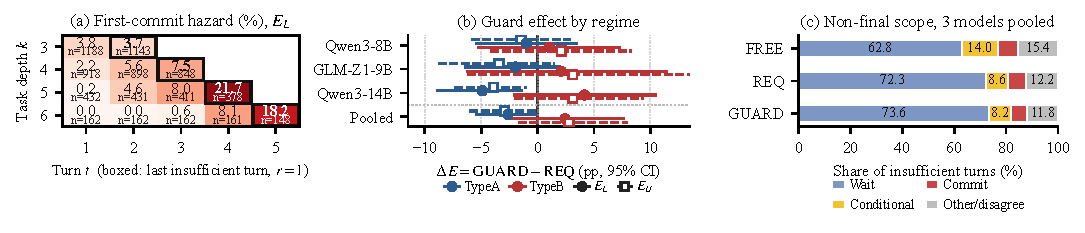
\includegraphics[width=\textwidth]{fig2_hazard_guard_scope.pdf}
    \caption{(a)~First-commit hazard $h(t,k)$ ($E_L$, pooled over models/protocols; $n$ = at risk; boxed: $r{=}1$). (b)~Guard effect $\Delta E{=}$\pGRD$-$\pREQ{} by regime with 95\% bootstrap CIs (solid: $E_L$, dashed: $E_U$). (c)~Non-final scope shares.}
    \label{fig:scope_hazard}
\end{figure*}

\textbf{Hazard escalates in later turns.} Pooled confirmed first-commit hazard rises $2.4\%$ ($t{=}1$) to $17.6\%$ ($t{=}4$); per protocol, ${\le}0.5\%$ ($r{=}4$) to $8.0\%$--$8.9\%$ ($r{=}1$; $E_U$ $9.5\%$--$11.6\%$). Fig.~\ref{fig:scope_hazard}(a) separates both: within fixed $k$ the rise is steep ($k{=}5$: $0.2\%\to4.6\%\to8.0\%\to21.7\%$), while fixed-$t$ dependence on $r$ is mixed ($t{=}2$: $3.7\%$/$5.6\%$/$4.6\%$; $t{=}4$: $21.7\%$ vs.\ $8.1\%$). The baseline hazard model gives $\beta_t{=}0.85$ (fixed-$k$ joint turn+proximity odds ${\times}2.33$, 95\% CI $[1.73,3.27]$), $\beta_t{+}\beta_k{=}0.51$ (fixed-$r$ turn odds ${\times}1.66$ $[1.17,2.45]$), and $\beta_k{=}{-}0.34$ (fixed-$t$ odds ${\times}0.71$ $[0.53,0.97]$; same pattern under $E_U$). Adding regime/topic (G1--G4) covariates gives $\beta_t{=}0.87$ (OR $2.39$) and $\beta_t{+}\beta_k{=}0.62$ (OR $1.86$ $[1.35,2.86]$), with $\beta_k$ non-significant ($[-0.60,+0.15]$); dropping $k{=}6$ ($N{=}94$) or 88 lexically matched trajectories keeps both positive ($\beta_t{+}\beta_k$ OR $2.21$/$1.77$, $>1$), while in non-matched \TA{} ($N{=}68$) $\beta_t$ stays positive (OR $1.80$ $[1.30,2.76]$) and $\beta_t{+}\beta_k$ crosses zero ($[-0.10,+0.91]$). Late escalation thus reflects joint turn-and-proximity growth; mechanically, trajectory $E$ rises with depth ($7.3\%$--$10.1\%$ at $k{=}3$ vs.\ $31.5\%$--$36.6\%$ at $k{=}5$).

\begin{table*}[!t]
\centering
\caption{Non-final scope distribution (852 insufficient turns per cell; Dis./Oth.\ = non-commit judge disagreements, Partial/Other, Unresolved, and $<0.3\%$ empty truncations), regime-stratified $E$ and $Y{-}J$ ($[L,U]$, \%), and unprompted explicit retraction among $E_U{=}1$ trajectories (confirmed by both judges / flagged by either / $n$). Pooled retraction: $4/26/489$ ($0.8\%$--$5.3\%$).}
\label{tab:exp3_mechanism}
\footnotesize
\setlength{\tabcolsep}{3.6pt}
\renewcommand{\arraystretch}{0.96}
\begin{tabular}{@{}llcccccccc@{}}
\toprule
Model & Protocol & Wait & Cond. & Commit & Dis./Oth. & \TA{} $E$ & \TA{} $Y{-}J$ & \TB{} $E$ & Retraction (both/any/$n$) \\
\midrule
\multirow{3}{*}{Qwen3-8B} & \pFREE & 63.6 & 14.3 & 8.5 & 13.6 & [13.2, 18.6] & [12.3, 16.7] & [25.0, 28.1] & 0 / 2 / 65 \\
 & \pREQ & 73.9 & 8.9 & 6.8 & 10.3 & [10.3, 13.7] & [9.8, 13.2] & [20.8, 24.0] & 0 / 2 / 51 \\
 & \pGRD & 77.3 & 6.3 & 6.2 & 10.1 & [9.3, 12.3] & [8.8, 11.8] & [21.9, 26.0] & 0 / 2 / 50 \\
\midrule
\multirow{3}{*}{GLM-Z1-9B} & \pFREE & 59.5 & 13.3 & 8.1 & 19.1 & [15.2, 18.6] & [13.7, 17.2] & [22.9, 27.1] & 0 / 1 / 64 \\
 & \pREQ & 70.0 & 7.7 & 7.4 & 14.9 & [13.2, 15.7] & [12.3, 14.2] & [18.8, 22.9] & 1 / 3 / 54 \\
 & \pGRD & 69.6 & 8.1 & 7.2 & 15.1 & [11.3, 12.3] & [9.8, 10.8] & [20.8, 26.0] & 0 / 5 / 50 \\
\midrule
\multirow{3}{*}{Qwen3-14B} & \pFREE & 65.4 & 14.6 & 6.6 & 13.5 & [10.8, 16.7] & [9.3, 15.2] & [21.9, 25.0] & 0 / 1 / 58 \\
 & \pREQ & 72.9 & 9.0 & 6.6 & 11.5 & [11.8, 13.2] & [11.3, 12.7] & [20.8, 25.0] & 2 / 6 / 51 \\
 & \pGRD & 73.7 & 10.2 & 6.0 & 10.1 & [6.9, 9.3] & [6.4, 8.8] & [25.0, 28.1] & 1 / 4 / 46 \\
\bottomrule
\end{tabular}
\end{table*}


\textbf{Current-answer requests shift \texttt{Conditional} to \texttt{Wait} (suggestive) and cut non-final tokens.} \pREQ{} leaves $Y$ and $E$ unchanged vs.\ \pFREE{} (Table~\ref{tab:paired_contrasts}). Across non-final turns ($n{=}2{,}556$/protocol), agreed \texttt{Wait} rises $62.8\%\to72.3\%$ and \texttt{Conditional} drops $14.0\%\to8.6\%$ (Fig.~\ref{fig:scope_hazard}c), cutting agreed \texttt{Commit}+\texttt{Conditional} by $6.3$~pp ($21.8\%\to15.5\%$, $[-8.1,-4.6]$; per-judge $-9.3$/$-7.2$~pp). Both judges agree per model ($+7.0$ to $+10.7$~pp \texttt{Wait}), though envelopes cross zero as the secondary judge maps borderline derivations to \texttt{Wait} more often. Across trajectories ($n{=}900$/protocol), those with ${\ge}1$ turn labeled \texttt{Commit}/\texttt{Conditional} by both judges fall $11.6$~pp ($45.4\%\to33.9\%$, $[-14.6,-8.8]$; per-judge $-12.4$/$-11.3$~pp). \pFREE{} uses ${\sim}20\%$ more completion tokens than \pREQ{} solely on non-final turns (2,084 vs.\ 1,557/turn; final 3,080 vs.\ 3,035), via more \texttt{Conditional} turns and longer replies.

\textbf{Unprompted retraction is rare (RQ3).} Of 489 $E_U{=}1$ trajectories, judges flag retraction in 4 (both) and 26 (either; $0.8\%$--$5.3\%$; $0.0\%$--$2.6\%$ \TA, $1.8\%$--$8.5\%$ \TB; 0 qualifications), concentrated in 12 items ($9/26$ on one extremum). Our 3-rater blind audit (Sec.~\ref{sec:exp4a}) confirms $[0,1]/26$ flagged trajectories (majority $1/26$, in \TB) and $0/74$ sampled controls ($0/50$ audited \TA{} trajectories). Across 81 changed boxed \TA{} commits (72/81, 88.9\%, end $Y{=}1$---silent $m{=}5{\to}2$ overwrites), 59/81 (72.8\%) cite prior derivations in CoT only.

\subsection{Turn-1 Guard by Regime (RQ4)}\label{sec:exp4b}
\textbf{Aggregate effect: small, not significant, no side effects.} Vs.\ \pREQ, \pGRD{} trims confirmed $E$ by $0.3$--$2.0$~pp and lifts $J$ by $1.3$--$1.7$~pp; aggregate envelope CIs cross zero (ruling out ${>}10$~pp), $Y$ shifts $-0.3$ to $+1.3$~pp, abstention stays $1.7\%$--$4.7\%$, and Qwen3 tokens drop $3.8\%$--$4.6\%$.

\textbf{By regime: lower $E$ on \TA, none on \TB.} On \TA, \pGRD{} lowers $E$ on all models ($E_L$: $-1.0$ to $-4.9$~pp; $E_U$: $-1.5$ to $-3.9$~pp), regime-significant on \texttt{Qwen3-14B} ($E_L$: $-4.9$ $[-8.8,-1.5]$; $E_U$: $-3.9$ $[-7.4,-1.0]$, though its cross-judge envelope $[-10.3,+1.0]$ spans 0; Table~\ref{tab:paired_contrasts}) and suggestive pooled ($E_L$: $-2.6$ $[-5.4,-0.2]$; $E_U$: $-2.9$ $[-6.0,0.0]$; Fig.~\ref{fig:scope_hazard}b), with non-significant pooled $J_L$ gain ($+3.3$~pp $[-0.3,+6.9]$; e.g., \texttt{ob-cee-3948}). On \TB, Guard shows no benefit (pooled $E_L$ $+2.4$ $[-2.4,+7.6]$; $E_U$ $+2.8$ $[-1.7,+8.0]$). Interaction $\Delta E_{\mathrm{TypeA}}{-}\Delta E_{\mathrm{TypeB}}$ is negative across definitions (pooled $E_L$: $-5.0$ $[-11.0,+0.5]$; $E_U$: $-5.7$ $[-11.8,-0.3]$; pri./sec.\ $-5.0$/$-5.8$)---regime-significant on \texttt{Qwen3-14B} ($-9.1$/$-7.0$~pp) and suggestive only on $E_U$/secondary when pooled. Counting \texttt{Commit}+\texttt{Conditional} removes the interaction ($-1.5$ $[-7.6,+4.8]$) and \TA{} effect ($-1.8$ $[-4.7,+0.8]$): Guard shifts \TA{} commits mainly to \texttt{Conditional} on \texttt{Qwen3-14B}/\texttt{GLM-Z1-9B} and to \texttt{Wait} on \texttt{Qwen3-8B} (cutting \texttt{Qwen3-8B} \TA{} trajectory \texttt{Commit}+\texttt{Conditional} by $5.9$~pp, $[-10.3,-1.5]$); cross-model regime specificity thus remains a suggestive hypothesis beyond \texttt{Qwen3-14B}.

\textbf{Interpretation.} \TA{} prefixes lack a parameter caught by uniqueness checks, whereas unique relaxed \TB{} optima pass them; completeness guards and repeated-prompt ablations (for residual $6.9\%$--$12.3\%$ \TA{} commits) remain untested.

\begin{table*}[!t]
\centering
\caption{Dual-LLM agreement on final correctness and scope (\texttt{gpt-6.1-sol} vs.\ \texttt{deepseek-v4.1-flash}; 0 parse failures). Commit $E$ is evaluated per dynamic trajectory ($n{=}900$/model; turn-level $\kappa_E{=}0.854$--$0.881$). On \textsc{Dev}~20, pooled $\kappa_Y{=}1.000$, $\kappa_E{=}0.924$ per trajectory / $0.918$ per turn, and scope $\kappa{=}0.616$--$0.758$.}
\label{tab:exp4a_calibration}
\footnotesize
\setlength{\tabcolsep}{3.8pt}
\renewcommand{\arraystretch}{0.96}
\begin{tabular*}{\textwidth}{@{\extracolsep{\fill}}lcccccc@{}}
\toprule
 & \multicolumn{2}{c}{Final $Y$} & \multicolumn{2}{c}{Commit $E$} & \multicolumn{2}{c}{4-class scope $C$} \\
\cmidrule(lr){2-3}\cmidrule(lr){4-5}\cmidrule(lr){6-7}
Model & Agree & $\kappa$ & Agree & $\kappa$ & Agree & $\kappa$ \\
\midrule
Qwen3-8B & 99.77\% & 0.984 & 96.22\% & 0.863 & 89.3\% & 0.730 \\
GLM-Z1-9B & 99.61\% & 0.977 & 97.00\% & 0.895 & 84.1\% & 0.630 \\
Qwen3-14B & 99.89\% & 0.987 & 96.67\% & 0.873 & 88.9\% & 0.724 \\
\bottomrule
\end{tabular*}
\end{table*}


\subsection{Judge Reliability and Blind Human Audit}\label{sec:exp4a}
On \textsc{Test}~100, judges agree on $99.61\%$--$99.89\%$ of final answers ($\kappa{=}0.977$--$0.987$), $96.22\%$--$97.00\%$ of trajectory commits ($\kappa{=}0.863$--$0.895$; turn $\kappa{=}0.854$--$0.881$), and $84.1\%$--$89.3\%$ of 4-class scope ($\kappa{=}0.630$--$0.730$; Table~\ref{tab:exp4a_calibration}). SymPy decides 3,177/5,400 final replies (58.8\%), matching judge consensus on 3,165/3,167 (99.94\%; both mismatches box unsimplified expressions) and siding with the secondary judge on 9/10 splits. Repair agreement ($94.8\%$--$96.4\%$) reflects the ${\le}5\%$ base rate~\cite{ref20} (PA $0.00$--$0.43$).

\textbf{Blind human audit: Scope-120.} The same three raters labeled hint-free blind interfaces; inclusion probabilities $\hat{\pi}_i$ under quota/deduplicated sampling use $50{,}000$ replays. Across 9 exhaustive strata covering all 7,668 non-final turns ($n{=}120$), binary \texttt{Commit} agreement is $90.6\%$ unweighted (Fleiss' $\kappa{=}0.797$, $\mathrm{AC1}{=}0.824$; external--author $90.4\%$ vs.\ author--author $90.8\%$) and $94.9\%$ under stratum-calibrated H\'{a}jek weights ($w_i{\propto}1/\hat{\pi}_i$, $\mathrm{AC1}{=}0.937$; 4-class $89.6\%$, $\kappa{=}0.692$). Human and judge bounds intersect on $99.3\%$ of H\'{a}jek turns (descriptive linearized $\mathrm{SE}{=}0.46\%$; unweighted $97.5\%$), with $98.6\%$ $h_L$--$e_L$ agreement ($\kappa{=}0.895$) and $90/93$ ($96.8\%$) match on unanimous turns. Dual-LLM prevalence ($[7.03\%,8.97\%]$) brackets the human majority ($8.93\%$, $\mathrm{SE}{=}0.66\%$), whereas $[h_L,h_U]{=}[7.85\%,15.52\%]$ ($\mathrm{SE}{=}0.57\%/2.83\%$) widens because the external rater marks borderline derivations as \texttt{Commit} more often ($14.2\%$ H\'{a}jek rate vs.\ $8.9\%$--$9.2\%$ for authors; $\kappa{=}0.60$--$0.65$ vs.\ judges [$0.59$ naive vs.\ secondary], $92.1\%$--$93.0\%$ agree, vs.\ authors' $\kappa{=}0.81$--$0.89$; HT and $N_h/n_h$ differ ${<}0.5$~pp). Within-bucket draws and item deduplication ($\pi_{ij}{=}0$ per item) cut co-inclusion, yet cross-bucket blocking and small quotas ($n_h{=}6$--$18$, zero-variance risk) break 95\% Wald coverage, keeping SEs descriptive.

\textbf{Blind human audit: Repair-100.} Across 26 flagged candidates and 74/457 sampled controls (plus 6 empty, $0/6$), unanimous agreement is $99.0\%$ ($\mathrm{AC1}{=}0.993$; external--author $99.0\%$ vs.\ $100.0\%$). Raters confirm $[0,1]/26$ flagged ($1/26$ per author, $0/26$ external; $[0,1]/4$ dual-pos, $0/22$ single-pos, \texttt{ob-cee-3335}, \TB) and $0/74$ controls ($0/50$ audited \TA)---giving $0.0\%$--$0.2\%$ HT point rates over all 489 $E_U{=}1$ runs, with no valid design-based 95\% bound under unequal $\hat{\pi}_j{\in}[0.079,0.303]$ and zero control hits (claims stay within the 100 cases; uncertified stress-test result in repo).

\section{Discussion, Limitations, and Conclusion}

\textbf{Design implications (hypotheses for CSCWD).} First, outcome scoring masks process failures ($9.3\%$--$17.2\%$ of \TA{} runs end $Y{=}1$ despite early commits). Second, repeated cues can separate attenuation from near-completeness. Third, given silent overwrites (72/81 changed boxed \TA{} commits end $Y{=}1$; $0/50$ audited \TA{} retractions), studies can test if retractions and scoped replies curb adoption ($m{=}5{\to}2$).

\textbf{Limitations.} (i)~\emph{Audit \& judging:} two of three raters are authors, so majority can reflect authors ($[L,U]$/per-rater labels take priority); 4-class scope is noisier; quota/deduplicated sampling leaves \emph{Scope-120} SEs descriptive without a valid \emph{Repair-100} 95\% bound (Guard echoes $<0.5\%$). (ii)~\emph{Benchmark:} SymPy checks formalized clauses, and strict fidelity varies ($[75,100]/100$); \TB{} mixes unbounded/finite relaxations; OlympiadBench admits contamination (lexical exclusion keeps $E$/$Y{-}J$, not non-verbatim recall). (iii)~\emph{Scope:} two 8B--14B families, scripted math, unadjusted CIs, and one exploratory guard (\texttt{Qwen3-14B} mainly; null with \texttt{Conditional}) support controlled decoupling, not larger models or live tasks.

\textbf{Conclusion.} Across 5,400 runs, 8B--14B reasoning LLMs commit under insufficiency, late and masked by $Y$; unprompted retraction is rare ($0.8\%$--$5.3\%$ flagged; $[0,1]/26$, $0/74$ human); and an exploratory guard yields modest, non-universal \TA{} gains (\texttt{Qwen3-14B} mainly, partly conditional).

{\scriptsize\def\IEEEbibitemsep{0pt plus 0.1pt}\begin{thebibliography}{00}

\bibitem{ref7} E. Horvitz, ``Principles of mixed-initiative user interfaces,'' in \textit{Proc.\ CHI}, 1999, pp. 159--166.
\bibitem{ref14} S. Amershi et al., ``Guidelines for human-AI interaction,'' in \textit{Proc.\ CHI}, 2019, pp. 1--13.
\bibitem{ref21} X. Zhao et al., ``A bio-inspired design method based on LLM: A case study of flying car concept design,'' in \textit{Proc.\ IEEE CSCWD}, 2025, pp. 2478--2483.
\bibitem{ref15} G. Bansal et al., ``Does the whole exceed its parts? The effect of AI explanations on complementary team performance,'' in \textit{Proc.\ CHI}, 2021.
\bibitem{ref23} T. R. G. Green, ``Cognitive dimensions of notations,'' in \textit{Proc.\ HCI'89}, Cambridge Univ.\ Press, 1989, pp. 443--460.
\bibitem{ref24} T. R. G. Green and M. Petre, ``Usability analysis of visual programming environments,'' \textit{J.\ Vis.\ Lang.\ Comput.}, vol. 7, no. 2, pp. 131--174, 1996.
\bibitem{ref25} D. G. Jansson and S. M. Smith, ``Design fixation,'' \textit{Des.\ Stud.}, vol. 12, no. 1, pp. 3--11, 1991.
\bibitem{ref6} C. He et al., ``OlympiadBench: A challenging benchmark for promoting AGI with olympiad-level bilingual multimodal scientific problems,'' in \textit{Proc.\ ACL}, 2024, pp. 3828--3850.
\bibitem{ref11} K. Cobbe et al., ``Training verifiers to solve math word problems,'' arXiv:2110.14168, 2021.
\bibitem{ref12} D. Hendrycks et al., ``Measuring mathematical problem solving with the MATH dataset,'' in \textit{Proc.\ NeurIPS}, 2021.
\bibitem{ref1} P. Laban, H. Hayashi, Y. Zhou, and J. Neville, ``LLMs get lost in multi-turn conversation,'' arXiv:2505.06120, 2025.
\bibitem{ref4} S. Luo et al., ``ClarifyMT-Bench: Benchmarking and improving multi-turn clarification for conversational LLMs,'' arXiv:2512.21120, 2025.
\bibitem{ref2} T. Chen, S. Wu, and J. Leskovec, ``Found in conversation: LLMs teach themselves to close the multi-turn gap,'' arXiv:2605.24432, 2026.
\bibitem{ref3} M. Li et al., ``Mitigating lost in multi-turn conversation via curriculum RL with verifiable accuracy and abstention rewards,'' in \textit{Proc.\ ACL}, 2026, pp. 33364--33381.
\bibitem{ref5} J. Su and J. Healey, ``Clarification is not enough: Post-clarification answering remains the bottleneck in multi-turn QA,'' arXiv:2605.25204, 2026.
\bibitem{ref27} B. Z. Li, B. Kim, and Z. Wang, ``QuestBench: Can LLMs ask the right question to acquire information in reasoning tasks?'' in \textit{Proc.\ NeurIPS}, 2025.
\bibitem{ref28} C. Fan, M. Li, L. Sun, and T. Zhou, ``Missing premise exacerbates overthinking: Are reasoning models losing critical thinking skill?'' arXiv:2504.06514, 2025.
\bibitem{ref29} Y. Huang et al., ``Do LLMs know what to ask and when? Evaluating multi-turn information seeking,'' arXiv:2608.14808, 2026.
\bibitem{ref8} S. Rao and H. Daum\'{e} III, ``Learning to ask good questions: Ranking clarification questions using neural EVPI,'' in \textit{Proc.\ ACL}, 2018, pp. 2737--2746.
\bibitem{ref9} A. Kamath, R. Jia, and P. Liang, ``Selective question answering under domain shift,'' in \textit{Proc.\ ACL}, 2020, pp. 5684--5696.
\bibitem{ref10} S. Kadavath et al., ``Language models (mostly) know what they know,'' arXiv:2207.05221, 2022.
\bibitem{ref26} J. Huang et al., ``Large language models cannot self-correct reasoning yet,'' in \textit{Proc.\ ICLR}, 2024.
\bibitem{ref16} A. Yang et al., ``Qwen3 technical report,'' arXiv:2505.09388, 2025.
\bibitem{ref17} Team GLM, ``GLM-Z1-9B-0414,'' Hugging Face (\texttt{zai-org/GLM-Z1-9B-0414}), Apr.\ 2025 (GLM-4 lineage: arXiv:2406.12793).
\bibitem{ref13} J. Wei et al., ``Chain-of-thought prompting elicits reasoning in large language models,'' in \textit{Proc.\ NeurIPS}, 2022, pp. 24824--24837.
\bibitem{ref19} A. Meurer et al., ``SymPy: Symbolic computing in Python,'' \textit{PeerJ Comput.\ Sci.}, vol. 3, e103, 2017.
\bibitem{ref18} W. Kwon et al., ``Efficient memory management for LLM serving with PagedAttention,'' in \textit{Proc.\ ACM SOSP}, 2023, pp. 611--626.
\bibitem{ref20} A. R. Feinstein and D. V. Cicchetti, ``High agreement but low kappa: I. The problems of two paradoxes,'' \textit{J.\ Clin.\ Epidemiol.}, vol. 43, no. 6, pp. 543--549, 1990.

\end{thebibliography}}

\end{document}
